% This line sets the project root file.
% 
% !TEX root = fib2.tex
% 
%------------------------------------------------------------------------------------------------------------%
% if we want to consider a PRL-style version, use these settings
\documentclass[aps, prl, letterpaper, twocolumn, superscriptaddress, notitlepage, 10pt]{revtex4-1}
\usepackage{times}

% use these settings for a more reader-friendly version
%\documentclass[aps, pra, a4paper, 11pt, onecolumn, nofootinbib, superscriptaddress, tightenlines, notitlepage, longbibliography]{revtex4-1}

% Packages, Macros, Layout, Environments, etc.
% This line sets the project root file.
% 
% !TEX root = ../fib2.tex
% 
%------------------------------------------------------------------------------------------------------------%

%------------------------------------------------------------------------------------------------------------%
% Packages
%------------------------------------------------------------------------------------------------------------%

\usepackage{color}
\usepackage{amsmath,amsfonts,amssymb,amsthm}
\usepackage{graphicx}
\usepackage{fullpage}
%\usepackage{caption}
\PassOptionsToPackage{caption=false}{subfig}
\usepackage{subfig}
\usepackage{enumerate}

\usepackage{tikz}
\usetikzlibrary{arrows,decorations.pathmorphing,backgrounds,positioning,fit}
%\usepackage[square,comma,numbers,sort&compress]{natbib}
\usepackage{epstopdf} % to include .eps graphics files with pdfLaTeX
\usepackage{bm}  % Define \bm{} to use bold math fonts

\usepackage[pdfpagelabels,pdftex,bookmarks,breaklinks]{hyperref}
\definecolor{darkblue}{RGB}{0,0,127} % choose colors
\definecolor{darkgreen}{RGB}{0,150,0}
\hypersetup{colorlinks, linkcolor=darkblue, citecolor=darkgreen, filecolor=red, urlcolor=blue}
%\hypersetup{pdftitle=Title\ Goes\ Here}% add a title to the metadata

\usepackage{layout}

%------------------------------------------------------------------------------------------------------------%
% PGF Stuff
%------------------------------------------------------------------------------------------------------------%

%\pgfrealjobname{main}

%------------------------------------------------------------------------------------------------------------%
% Page Layout
%------------------------------------------------------------------------------------------------------------%

\addtolength{\textheight}{0\textheight}

%------------------------------------------------------------------------------------------------------------%
% Theorem Environments
%------------------------------------------------------------------------------------------------------------%

\newtheorem{theorem}{Theorem}
\newtheorem{proposition}[theorem]{Proposition}
\newtheorem{lemma}[theorem]{Lemma}
\newtheorem{corollary}[theorem]{Corollary}
\newtheorem{definition}[theorem]{Definition}
\newtheorem{remark}[theorem]{Remark}
\newtheorem{example}[theorem]{Example}

\newtheorem{claim}{Claim}[section]

\renewenvironment{proof}[1][Proof]{\noindent\textbf{#1.} }{\ $\Box$}

%------------------------------------------------------------------------------------------------------------%
% Macros
%------------------------------------------------------------------------------------------------------------%

% double-struck math font
\def\N{\mathbb{N}}
\def\Z{\mathbb{Z}}
\def\R{\mathbb{R}}
\def\C{\mathbb{C}}
\def\E{\mathbb{E}}

\def\e{\mathrm{e}}
\def\lg{\mathrm{lg}}

\newcommand{\Eref}[1]{Eq.~(\ref{#1})}
\newcommand{\Sref}[1]{Sec.~\ref{#1}}
\newcommand{\Fref}[1]{Fig.~\ref{#1}}
\newcommand{\Aref}[1]{Appendix~\ref{#1}}

\def\eps{\epsilon}
\def\th{^{\rm th}}
\def\st{^{\rm st}}
\def\rd{^{\rm rd}}
\def\cO{\mathcal{O}}
\DeclareMathOperator{\Tr}{Tr}
\DeclareMathOperator{\tr}{tr}
\DeclareMathOperator{\Prob}{Prob}

\newcommand{\ket}[1]{|{#1}\rangle}
\newcommand{\expect}[1]{\langle{#1}\rangle}
\newcommand{\bra}[1]{\langle{#1}|}
\newcommand{\ketbra}[2]{|{#1}\rangle\!\langle{#2}|}
\newcommand{\braket}[2]{\langle{#1}|{#2}\rangle}
\newcommand{\proj}[1]{\ketbra{#1}{#1}}

%------------------------------------------------------------------------------------------------------------%
% Comment fonts
%------------------------------------------------------------------------------------------------------------%

\newcommand{\cggb}[1]{\textcolor{blue}{#1}}
\newcommand{\sdb}[1]{\textcolor{red}{#1}}



% use this for multiline block comments: \/* commented text here */
\long\def\/*#1*/{}
%\long\def\/*#1*/{#1} % uncomment this line to load the block comments

%------------------------------------------------------------------------------------------------------------%
\begin{document}

\title{Classical Simulation of Quantum Error Correction in a Fibonacci Anyon Code}

\author{Simon Burton}
\affiliation{Centre for Engineered Quantum Systems, School of Physics, 
The University of Sydney, Sydney, Australia}
\author{Courtney G.\ Brell}
\affiliation{Institut f\"{u}r Theoretische Physik, Leibniz Universit\"{a}t Hannover, 
Appelstra\ss{}e 2, 30167 Hannover, Germany}
\author{Steven T.\ Flammia}
\affiliation{Centre for Engineered Quantum Systems, School of Physics, 
The University of Sydney, Sydney, Australia}

\date{\today}

\begin{abstract}
Classically simulating the dynamics of excitations in two-dimensional quantum systems that support anyons is likely intractable in general because such dynamics are sufficient for universal quantum computation. However, for typical processes of interest for the the study of quantum error correction in anyon systems, the relevant dynamics can in fact be efficiently simulated classically for a wide range of system parameters, even when the underlying anyon model is universal~\cite{RGsim}. We make use of this fact to demonstrate the success of an error-correction protocol for a Fibonacci anyon quantum memory. We numerically simulate a phenomenological model of the system and noise processes on lattice sizes of up to $128\times128$ sites, and find a lower bound on the error-correction threshold of approximately $12.5\%$, which is comparable to those previously known for abelian and (non-universal) nonabelian anyon models.
\end{abstract}

\maketitle

%------------------------------------------------------------------------------------------------------------%

Anyonic excitations in two-dimensional quantum systems~\cite{Wilczek1990} offer 
tremendous promise for long-term storage and processing of quantum 
information~\cite{Kitaev2003}. The topological features of quantum systems that support 
such excitations are insensitive to local 
perturbations~\cite{Bravyi2010, *Bravyi2011a, *Michalakis2013}, and the excitations 
themselves can in general be used to perform universal quantum 
computation~\cite{Freedman2002, *Freedman2002b}. 

Quantum error correction is vital to harnessing the computational power of these topologically 
ordered systems. When coupled to a heat bath at any finite temperature, thermal fluctuations 
will create anyons that diffuse and quickly corrupt the stored quantum 
information~\cite{Pastawski2010}. Thus, the passive protection provided by the mass gap 
and low temperature must be augmented by an \emph{active} procedure. 

Almost all of the sizable research effort on active quantum error correction for topological 
systems has focused on the case of abelian anyons~\cite{Terhal2014}. These systems are 
well suited to studying quantum error correction because the dynamics of excitations in 
abelian anyon models can be simulated numerically very efficiently, allowing lattice 
simulations of decoding with over 1 million sites~\cite{Duclos-Cianci2010}. The ability to 
efficiently simulate these systems is a consequence of the limitation that abelian anyons 
cannot be used for universal quantum computation. 

Recent investigations have begun to explore quantum error correction for nonabelian anyon 
models~\cite{Brell2013, Wootton2013, Hutter2014}. These models are particularly interesting 
because braiding and fusion of anyons in these models leads in general to universal quantum 
computation. However, the initial studies have focused on models such as Ising 
anyons~\cite{Brell2013} and the so-called $\Phi$-$\Lambda$ 
model~\cite{Wootton2013, Hutter2014} that, while nonabelian, are not universal, a fact 
that was exploited to enable efficient classical simulation of error correction in these systems. 
The remarkable computational power of universal anyon models becomes a liability when we 
seek to simulate these systems on classical computers. 

Here we consider a full simulation of quantum error correction in a two-dimensional lattice 
system with Fibonacci anyons, a class of nonabelian anyons that are universal for quantum 
computation~\cite{Wang2010b}. Fibonacci anyons are experimentally motivated as the 
expected excitations of the $\nu=\frac{12}{5}$ fractional quantum Hall 
states~\cite{Slingerland2001}, and can also be realized in several spin 
models~\cite{Levin2005, Kapit2013, Palumbo2014} and composite heterostructures~\cite{Mong2014}.

\stf{Describe main results and why they are badass. cite:~\cite{Bonesteel2012}}

%------------------------------------------------------------------------------------------------------------%
\paragraph{Modelling Fibonacci anyons.}

The topological features of a physical anyon model are abstractly described by a unitary modular tensor category~\cite{Wang2010b}. This object contains the data describing the types of anyonic particles, as well as the results of topological operations such as braiding or fusion of these anyons. The Fibonacci anyon model consists of only one non-trivial particle type, conventionally labelled $\tau$. Denoting the vacuum by $\mathbb{I}$, we can describe the possible fusion outcomes of Fibonacci anyons as $\tau\times\tau=\mathbb{I}+\tau$, i.e.~two $\tau$ particles can either fuse to vacuum or to a $\tau$ particle.

Associated with each set of fusion outcomes for a fixed number of $\tau$ particles is a basis vector for a Hilbert space, the \emph{fusion} space. For $n$ particles of type $\tau$, the dimension of this space grows asymptotically as $\varphi^n$ for $\varphi=\frac{1+\sqrt{5}}{2}$ the golden ratio. Additionally, there is a global degeneracy associated with the topology of the manifold on which the anyons reside. We will consider systems with the topology of a torus, which for the Fibonacci anyons gives rise to a 2-fold degeneracy. For convenience (in particular to minimize finite-size effects in our numerical computations~\cite{Brell2013}), this global space is the one in which we will encode, and demonstrate protection of, quantum information.
	
The fusion outcome of any particular experiment depends on the history of the particles, in particular how they have braided around one another. Braiding operations are treated as unitary actions on the fusion space. Pair-creation events should be considered isometries that enlarge the fusion space, while fusion events correspond to projective 
measurements of combined charge of some number of particles. For details of the description of these processes in Fibonacci anyons, see Ref.~\cite{Trebst2008}. \stf{check that this ref is a good one...} Braiding of Fibonacci anyons and measurements of fusion outcomes is known to be sufficient to implement universal quantum computation~\cite{?}.

We use a phenomenological model of Fibonacci anyon dynamics which neglects any microscopic details of the system. This is consistent with the principles of topologically ordered systems and anyonic physics, where the key universal features describing the anyon model correspond to large length-scale physics, while the microscopic physics plays a less 
important (and non-universal) role. As such, we model the system simply as a periodic $L\times L$ square lattice $\Lambda$ of sites with upon which sets of anyons can reside. Allowed anyon dynamics (pair-creation, braiding, and fusion) are considered to act locally on edges of $\Lambda$. For more details of an analogous model, see~\cite{Brell2013}.
	
%------------------------------------------------------------------------------------------------------------%
\paragraph{Noise and error-correction.}

	We consider encoding a qubit of quantum information in the global degeneracy associated with the topology of the manifold of our system. We imagine an idealized Hamiltonian for this system of the form
	\begin{align}
		H=-\sum_{i\in \Lambda}\proj{\mathbb{I}}_i\;,\label{e:hamiltonian}
	\end{align}
with $\proj{\mathbb{I}}_i$ the projector to charge $\mathbb{I}$ at site $i$, i.e.~the ground space of the model has vacuum (or no anyon) at each site. Given the toroidal boundary conditions, this space is two-fold degenerate as noted above. We identify this ground space as the codespace of our model. Typical realistic noise processes in this kind of system are pair-creation, hopping, exchange etc.~of anyons on neighbouring sites of $\Lambda$. It was seen in~\cite{Brell2013} that a simplified noise model consisting of pair-creation events only is sufficient to capture the qualitative features of an error-correction simulation, and so we will restrict to pair-creation noise processes in this study for convenience. These events act on neighbouring pairs of sites, and so may be associated with an edge of the lattice, chosen uniformly at random at each timestep of the simulation. The simulation time, and thus the error-correction threshold, will be measured in terms of average number of noise processes per edge, as opposed to an iid noise probability per edge. The latter measure is not appropriate for error processes in nonabelian anyon models, but the two coincide in the limit of low error rates in those cases where they are comparable (see Ref.~\cite{Brell2013}).

	In order to perform a logical error on our code, a noise process must have support on a ribbon running around a homologically nontrivial loop of the lattice. These correspond to processes in which anyonic charge is transported around the non-trivial loop before annihilating to vacuum. More details can be found in Ref.~\cite{?}.

	Our error-correction algorithm is based on the hard-decision renormalization group (RG) decoders studied in Refs.~\cite{?}. Our decoder proceeds by measuring the occupations of anyons at each site of the lattice, forming clusters of nearby anyons and fusing the anyons within each cluster, before iterating at increasing length scales. It terminates when the lattice is free of anyons (i.e.~we have returned to the codespace) or the clustering length scale exceeds the total size of the lattice. \cggb{A few more details? What is our length schedule?} \cggb{How does our decoder relate to other decoding schemes used in~\cite{Wootton2013,Brell2013,Hutter2014}?} Note that we expect that our qualitative results may be reproduced by most alternative families of decoders, such as matching decoders~\cite{?} and soft-decisions RG decoders~\cite{?} \cggb{do we?}. The advantage of using a hard-decision RG decoder is its simplicity and flexibility, and the fact that this simplicity allows for a proof of efficient classical simulability of successful error-correction~\cite{RGsim}.

\begin{figure*}[th!]
\begin{center}
	{\scriptsize (i)
	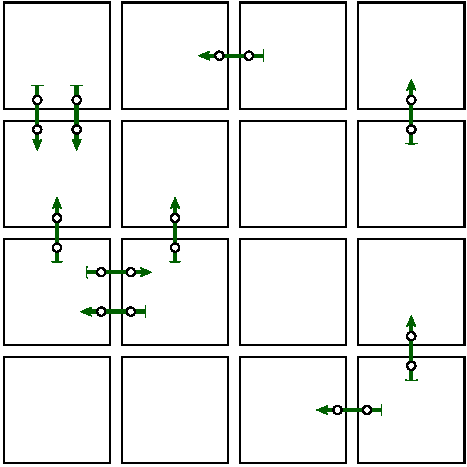
\includegraphics[width=0.57\columnwidth]{pair-create.pdf}
	\hskip 4pt
	(ii)
	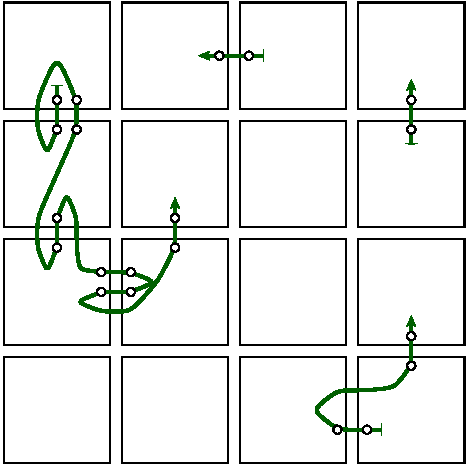
\includegraphics[width=0.57\columnwidth]{syndrome-1.pdf}
	\hskip 4pt
	(iii)}
	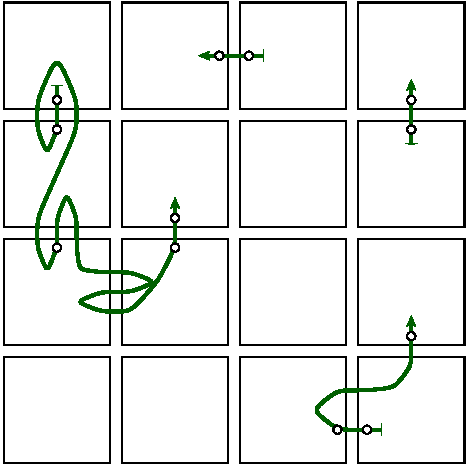
\includegraphics[width=0.57\columnwidth]{syndrome-2.pdf}
\caption{The simulation of noise processes proceeds by i) creating pairs of anyons on neighbouring tiles represented by open curves ii) joining the curves within a given tile iii) measuring the total charge on each tile.}
\label{f:simex}
\end{center}
\end{figure*}
	
%------------------------------------------------------------------------------------------------------------%	
\paragraph{Classical simulability.}

Although simulating pair creation, braiding, and fusion of $n$ Fibonacci anyons is equivalent in computational power to universal quantum computing (and thus unlikely to be classically tractable), noise processes and error-correction procedures have structure that we can exploit to efficiently simulate typical processes of interest~\cite{RGsim}. In particular, those processes in which we expect error-correction to succeed are also those that we expect to be able to efficiently 
simulate for the following heuristic reasons (see Ref.~\cite{RGsim} for a more rigorous analysis).

Below the (bond) percolation threshold for (say) a square lattice, we expect random sets of bonds to decompose into separate clusters of average size $O(\log(n))$ and variance $O(1)$~\cite{Bazant2000}. \cggb{Do we want to use the word cluster here again or switch?} Each noise process in our model is associated with a (randomly distributed) edge, and so disconnected clusters correspond to sets of anyons that could not have interacted at any point in their history. As such, we can simulate the braiding processes of each cluster separately. In other words: the quantum state in the fusion space of all anyons factorizes into a tensor product over bond clusters, and we can compute each factor separately. Since each cluster has size only $O(\log(n))$, we can typically simulate these dynamics efficiently because the resulting fusion space has dimension $O(\mathrm{poly}(n))$. There are rare random processes that violate this reasoning, but processes such as these are suppressed exponentially in $L$, the lattice size~\cite{Grimmett1989}. 

However, random noise processes are not the only dynamics that we need to consider. We must also consider the effect of the error-correction routine itself. This acts iteratively to fuse particles on increasing length scales. While this kind of fusion would typically merge clusters, forcing us to compute dynamics of larger and larger sets of anyons, large clusters are sparse (and thus unlikely to be merged), and in addition at each length scale the total number of anyons present is dramatically reduced by fusion, leading to a smaller number of anyons that must be simulated.

Of course, if we were to consider noise so strong that the clusters percolate over the lattice, we would no longer be able to efficiently simulate the system. However, recall that logical errors in our system correspond to processes that act over a non-trivial loop of the torus. If the noise operations are so common to have percolated, this is an example of a situation where we expect error-correction \emph{not} to succeed. Similarly, if the noise has not yet percolated by itself, but the clusters are merged into a large (percolated) cluster by the decoding algorithm, this is again an example of a process that we expect to correspond to a failure of error-correction. In this way, we see that the events that we are able to efficiently simulate correspond precisely to those for which we expect error-correction to succeed. We can simply declare failure on non-simulable events. This allows us to simulate and demonstrate the success of error-correction schemes for Fibonacci anyons, without explicitly simulating the failure of such schemes.

%------------------------------------------------------------------------------------------------------------%	
\paragraph{Simulation algorithm.}

	Our concrete simulation proceeds by associating a \emph{tile} with each site of the $L\times L$ periodic square lattice. In order to keep track of the observables of the system we maintain a set of disjoint curves, representing the history of anyons on the lattice (these curves can also be thought of as a top-down view of the fusion tree). The ends of curves correspond to leaves of the fusion tree, or anyons. In general, the curves wind around the two dimensional tiles in a haphazard way determined by the progress of the simulation. This allows a dynamically generated basis for the fusion space that easily allows for tensor decomposition into factors corresponding disjoint clusters. For comparison, previous work used a single fixed basis for the fusion space (determined by row-major ordering of sites)~\cite{Brell2013}.

Each round of simulation proceeds in four steps as follows (an example is shown in \Fref{f:simex}).

\begin{enumerate}[i)]
	\item The noise process is modelled by a sequence of pair-creation events distributed as a Poisson process across each edge. Curves are created crossing the relevent edge and terminating on the neighbouring sites.
	\item We first join curves that participate in the same tile in order to, \cggb{maybe a couple more lines of detail on this and the next point?}
	\item measure the charge on each tile. Any resulting anyon is left somewhere in the tile.
	\item The decoder examines this syndrome and clusters nearby anyons. Each cluster is then measured (fused), and the decoder continues to cluster and fuse on larger scales until there are no more anyons, or a cluster includes a non-trivial loop on the lattice. Since operators with support on such non-trivial clusters will generally perform an undetectable error on the encoded state, in this case we abandon the simulation and declare failure to error correct.
\end{enumerate}

%------------------------------------------------------------------------------------------------------------%
\paragraph{Numerical results.}

	We plot the performance of the decoder as a function of error rate for varying lattice sizes in \Fref{f:threshold}. The error rate is parameterized by the Poisson process duration $t_{\mathrm{sim}}$, representing the expected number of errors per edge over the simulation. We find evidence of a decoding threshold below which decoding succeeds with asymptotic certainty as the system size increases at $t_{\mathrm{sim}}\simeq 0.125 \pm 0.003$.

\begin{figure}[th!]
\begin{center}
	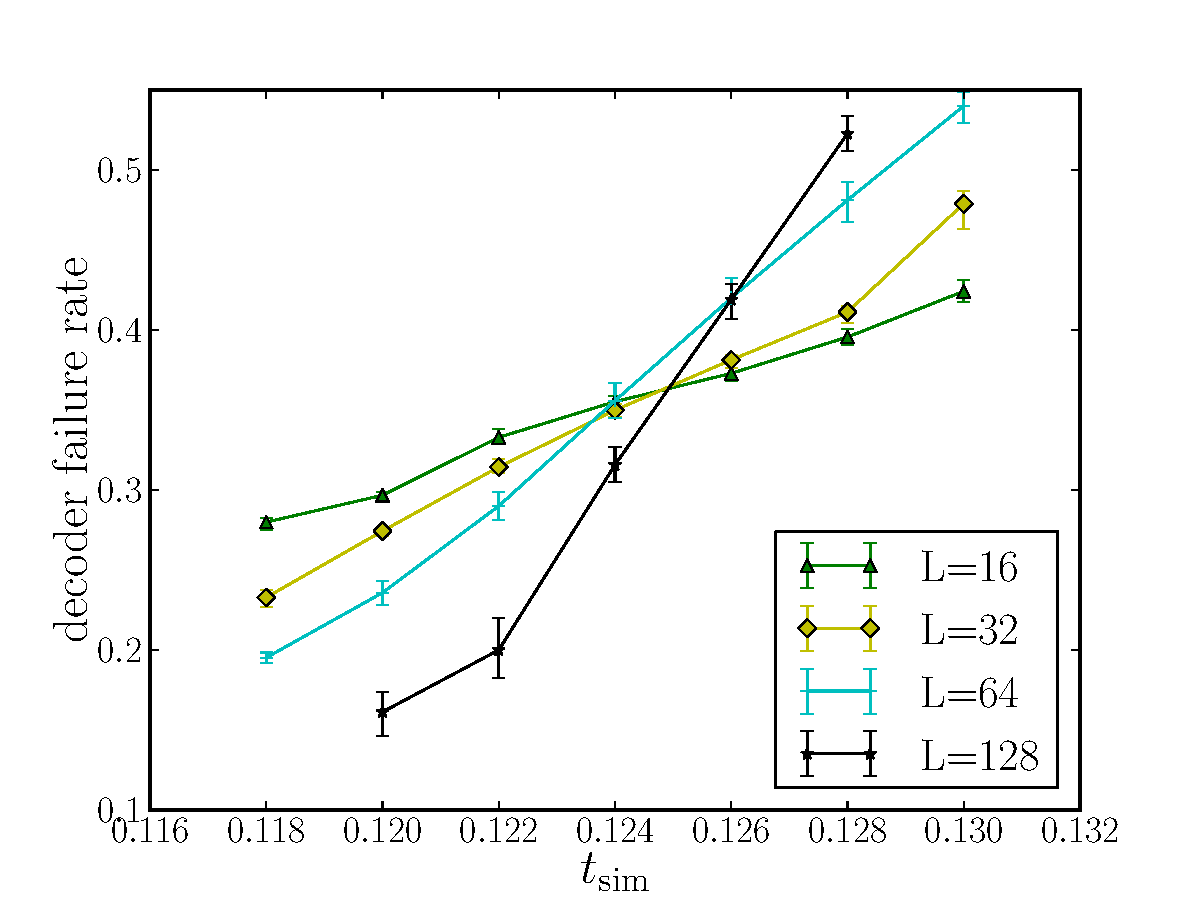
\includegraphics[width=\columnwidth]{anyons-kyle.pdf}
\caption{Decoder failure as a function of simulation time for various lattice sizes, showing threshold behavior around at $t_{\mathrm{sim}}\simeq 0.125$.}
\label{f:threshold}
\end{center}
\end{figure}


\cggb{Do we need to define $t_{\mathrm{sim}}$ more explicitly?}
	
\cggb{Comment on the effect of declaring failure on some simulations on this plot. Would we expect it to change if we simulated every event completely? If so, how?}

%------------------------------------------------------------------------------------------------------------%
\paragraph{Discussion.}

	We have demonstrated classical simulation of successful error correction in a universal anyon model. Though we have chosen several properties of our model and simulation in a convenient way for simplicity, we think it very unlikely that they will affect the qualitative results, similarly to the results of Ref.~\cite{Brell2013}. In particular, although we have modelled our logical qubit as encoded in the global topological degrees of freedom of our system, we could have encoded it in the fusion space of several preferred $\tau$ anyons. This situation would be appropriate to model error-correction routines in a topological quantum computation protocol. Additionally, we expect our results to be stable to changes in details of the noise model, decoding algorithm, etc.
	
	None of our techniques are restricted to simulation of Fibonacci anyon dynamics, and could equally well be used to simulate successful error-correction protocols in an arbitrary anyon code.	
	
\cggb{Comment on applicability of our simulation techniques to non-phenomenological models. Is it possible that the same ideas could be useful when there is more microscopic detail available, or are they restricted to exactly our phenomenological setup?}

\stf{Is there a possibility of using MPS like Rob Pfeiffer to improve the simulations or include interactions?}

\cggb{Do we have much more to say?}


%------------------------------------------------------------------------------------------------------------%
\acknowledgements 

\cggb {People we chatted to.} This work was supported by the ARC via EQuS project number CE11001013, and by the US Army Research Office grant numbers W911NF-14-1-0098 and W911NF-14-1-0103. STF also acknowledges support from an ARC Future Fellowship FT130101744. \cggb{CGB funding.}

%------------------------------------------------------------------------------------------------------------%
%\bibliographystyle{bibstyle}
\bibliography{refs2}

\end{document}
